% vim: tw=80 sw=2 ts=2 ff=unix spelllang=en spell
\documentclass{beamer}
\newcommand{\colA}[1]{\begin{columns}[t]\begin{column}{#1}}
\newcommand{\colB}[1]{\end{column}\begin{column}{#1}}
\newcommand{\colEnd}{\end{column}\end{columns}}

\usetheme{CambridgeUS}
\usecolortheme{dolphin}
%\setbeamercovered{transparent}
%\useoutertheme{infolines}

\usepackage{xltxtra}
\usepackage{fancyvrb}
%% \usepackage{ngerman}
\institute[]{Centrum für Informations- und Sprachverarbeitung (CIS)\\
            Ludwig-Maximilians-Universität München (LMU)\\
            \vspace{1cm}
            \href{https://creativecommons.org/licenses/by-nc-sa/4.0/}%
            {\includegraphics[width=0.2\textwidth]{../presentations/images/by-nc-sa.eps}}}

% keine Navigationspfeile
\setbeamertemplate{navigation symbols}{} % keine Navigations-Buttons

% Standardschrift verändern für Griechisch
%\setsansfont[Mapping=tex-text]{Junicode}
%\setmonofont[Mapping=tex-text]{DejaVu Sans Mono}
%\setsansfont[Mapping=tex-text]{Linux Libertine O}
%\setsansfont[Scale=MatchLowercase]{Linux Biolinum O}

% Fußzeile mit Titel und Seitenr.
\definecolor{mygray}{gray}{0.25}
%\setbeamertemplate{footline}[frame number]
\setbeamertemplate{footline}{\color{mygray}\hspace*{2mm}\insertauthor\hfill \insertshorttitle\hfill\insertdate\hspace*{10pt}\insertframenumber\ / \inserttotalframenumber\hspace*{2ex}}

% Schrift für URLs
\definecolor{myblue}{rgb}{0.2 0.0 0.8}

\usepackage{hyperref}
\renewcommand{\UrlFont}{\color{myblue}\footnotesize\sf}
\hypersetup{colorlinks,allcolors=.,urlcolor=blue}

% Bibliography
%\usepackage[backend=biber,style=authoryear,maxcitenames=2,maxbibnames=9]{biblatex}

% Schriftgröße Listings
\RequirePackage{fancyvrb}
\DefineVerbatimEnvironment{Highlighting}{Verbatim}%
  {commandchars=\\\{\},fontsize=\footnotesize}
\DefineVerbatimEnvironment{Verbatim}{Verbatim}%
  {fontsize=\footnotesize}
\newcommand{\pocoto}{\texttt{PoCoTo}}

\title{DATeCH 2017 -- \pocoto{} Workshop -- \pocoto{}}
\author{Florian~Fink \& Uwe~Springmann}

\begin{document}

\begin{frame}
	\titlepage
\end{frame}

\section{Introduction to post-correction}
\subsection{Motivation}
\begin{frame}
	In the resent years a lot of historical documents have been
	scanned and OCR'ed.

	\begin{itemize}
		\item The overall quality of the character recognition on historical
			documents is in general good.
		\item The performance of the OCR engines even on historical documents has
			constantly improved.
		\item In some cases the quality can be further improved, by further
			adapting the original images and OCR engines.
		\item But still the quality of the recognition is not good enough for
			deeper scientific studies on the documents.
	\end{itemize}
\end{frame}


\subsection{Text recognition on historical documents}
\begin{frame}
	\centering{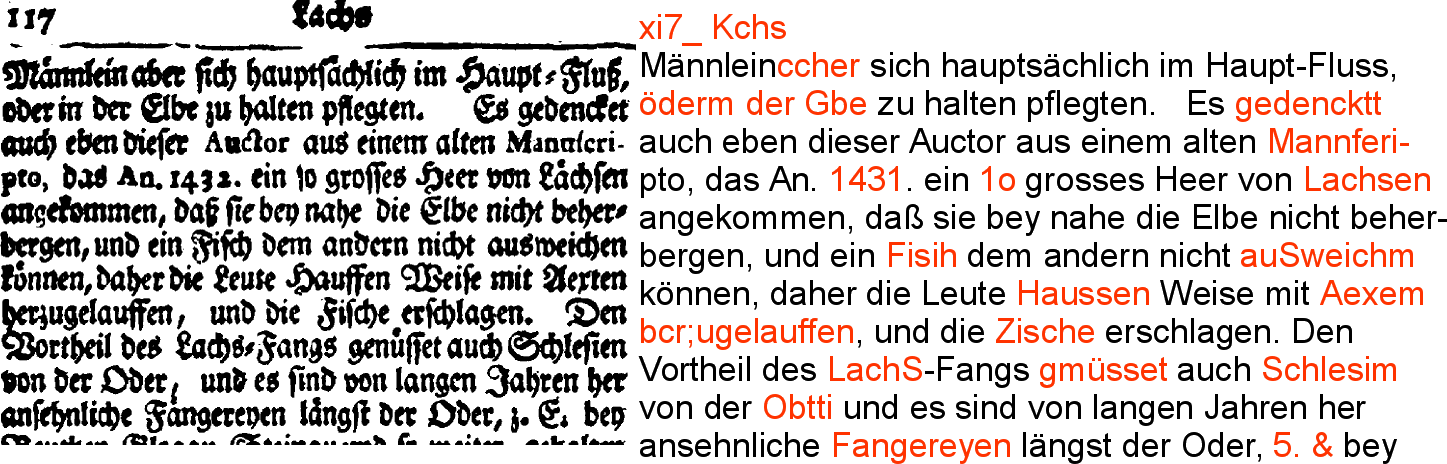
\includegraphics[width=\linewidth]{../presentations/images/hist_spellings2.png}}
	Example of the OCR results of a snippet of the \emph{BSB Zedlersches
	Universallexikon: article about salmon.}
\end{frame}

\subsection{Characterise recognition rates}
\begin{frame}
	\begin{table}
		\begin{tabular}{c c c c c}
			Year & Language & ABBYY FR 11.1 & Tesseract 3.03 & OCRopus 0.7 \\\hline
			1544 &   lat.   &    83,14      &     70,32      &      74,59 \\
			1649 &   lat.   &    88,07      &     84,87      &      78,98 \\
			1746 &   dt.    &    97,00      &     91,48      &      95,70 \\
			1779 &   lat.   &    82,13      &     80,77      &      75,46 \\
			1871 &   dt.    &    98,12      &     95,94      &      97,40 \\
		\end{tabular}
	\end{table}

	The results of the text recognition must be manually improved:
	\begin{itemize}
		\item Manual (double) keying of the original sources is expensive.
		\item Interactive postcorrection can be used examine the results of the
			OCR.
		\item Interactive postcorrection can be used to improve the results of the
			OCR.
	\end{itemize}
\end{frame}

\section{\pocoto{} -- The PostCorrectionTool}
\subsection{Overview}
\begin{frame}
	\centering{
\includegraphics[width=0.5\linewidth]{../presentations/images/impact.png}}
	\begin{itemize}
		\item \pocoto{} is a tool for the interactive post-correction of OCR'ed
			text:
		\item It was developed as part of the EU founded project IMPACT.
		\item It is open source and hosted on
			\href{https://github.com/cisocrgroup/PoCoTo}{github}.
		\item It contains linguistic and visual aids to support the post-correction.
		\item It contains aids to automatically correct systematic errors in the
			documents.
		\item You find its documentation in the
			\href{https://github.com/cisocrgroup/Resources/blob/master/manuals/pocoto-manual.md}{\pocoto{}
			manual} (included in this workshop's data package).
	\end{itemize}
\end{frame}

\subsection{Features}
\begin{frame}
	\begin{itemize}
		\item \pocoto{} has an automatic update mechanism -- once installed, it is
			automatically kept up to date.
		\item The recognition results are visualized with the images of the original
			documents.
		\item The concordance views enable to examine different errors and error
			pattern over the whole document.
		\item A specialized profiling web-service can be used to get correction
			suggestions for unknown words and frequent error patterns in the document.
		\item Different formats can be read, manually corrected and written back.
	\end{itemize}
\end{frame}

\section{\pocoto{} -- Installation}
\subsection{Installation}
\begin{frame}
	\begin{itemize}
		\item You can download the application data file \texttt{ocrcorrection.zip}
			from \href{http://www.cis.lmu.de/ocrworkshop/pocoto/}{this link} or use
			the version that is part of this workshop's data package.
		\item Extract the archive to a convenient place
		\item Go to \texttt{ocrcorrection/bin} in the extracted directory and double click
			on the executable file \texttt{ocrcorrection} (Linux) or
			\texttt{ocrcorrection.exe} (Windows).
		\item You can create a link to this executable on your desktop for
			easier access.
	\end{itemize}
\end{frame}

\subsection{Updating}
\begin{frame}
	\begin{itemize}
		\item \pocoto{} has an automatic updating mechanism.
		\item \pocoto{} can be kept up to date without having to install it again.
		\item Whenever \pocoto recognizes a newer version, it shows an \emph{updates
			available} 
\includegraphics{../presentations/images/update-baloon.png}
			button in its lower right corner.
		\item To check for updates go to \texttt{Help->Check for updates}.
		\item To control the update go to \texttt{Tools->Plugins}.
	\end{itemize}
\end{frame}

\section{Graphical UI}
\subsection{The main areas}
\begin{frame}
	\centering{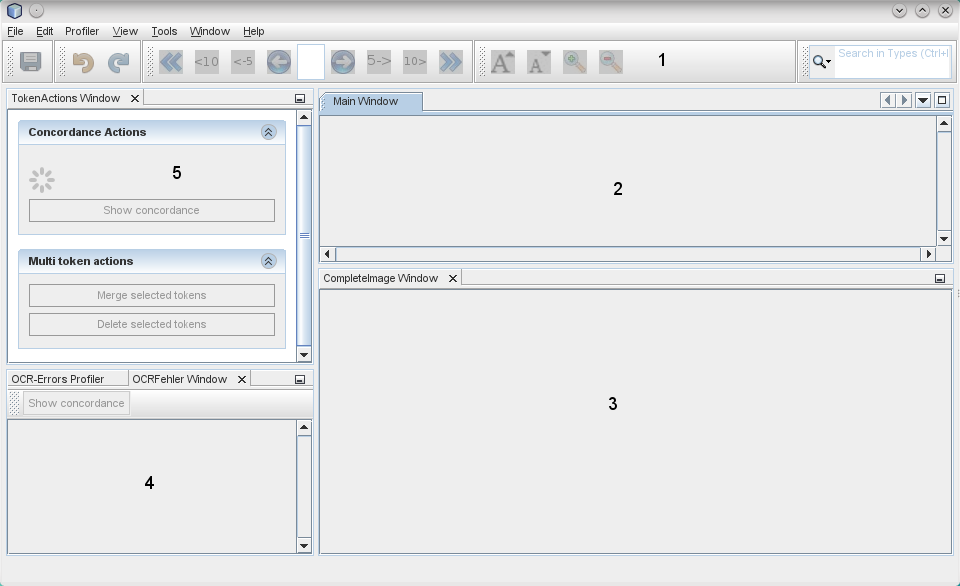
\includegraphics[width=\linewidth]{../presentations/images/pocotomainwindow_marked.png}}
\end{frame}

\subsection{The main areas}
\begin{frame}
	\pocoto{} is composed by 5 main areas. The size of each area can be
	freely adjusted:
	\begin{enumerate}
		\item The menu area contains various commands for navigation and project
			maintenance.
		\item The main view area shows tokens and offers the main correction
			possibilities.
		\item The complete image area displays the page of the current active
			(selected) token.
		\item The error area lists error frequency lists of common word or
			pattern errors.
		\item The token actions area lets you create concordance views an helps
			you to split and merge tokens.
	\end{enumerate}
\end{frame}

\section{\pocoto{} -- Projects and profiles}
\subsection{\pocoto{} project structure}
\begin{frame}
	\begin{itemize}
		\item \pocoto{} handles your input documents as separate projects
		\item Each project is constructed over a set of different files:
			\begin{itemize}
				\item The XML output files of your OCR engine.
				\item The image input files of your documents -- the same that you
					used for your OCR.
			\end{itemize}
		\item \pocoto{} expects those files to be organized in a specific way:
			\begin{itemize}
				\item All the XML files for your project should be in one folder
				\item All the image files for your project should be in another
					folder.
				\item Each image file should have the same name as its corresponding
					XML
					file, except for the file's extension (\texttt{.xml},
					\texttt{.png}, ...).
			\end{itemize}
		\item It is more convenient to have the two folders for your XML and image
			files together in one place and use this folder as base path for
			your project.
	\end{itemize}
\end{frame}

\subsection{\pocoto{}'s file formats}
\begin{frame}
	\pocoto{} understands three different XML file formats, that you can use
	to create new projects.
	\begin{enumerate}
		\item The character based ABBYY-XML format.
		\item The hOCR file format.
		\item Ocropus-Directories.
	\end{enumerate}
	\pocoto{} uses the information of the ABBYYX-XML file format directly to mark
	\emph{suspicious} words. It will generate an error frequency list for you. If
	you use the hOCR format or Ocropus, \pocoto{} is not able to generate such an
	error frequency list for you.
\end{frame}

\subsection{Creating a new project}
\begin{frame}
	\centering{\includegraphics<1-2>[height=.4\textheight]{../presentations/images/newprojectwizardstep1.png}}
	\centering{\includegraphics<3>[height=.4\textheight]{../presentations/images//newprojectwizardstep2.png}}
	\centering{\includegraphics<4>[height=.4\textheight]{../presentations/images/newprojectwizardstep3.png}}

	\begin{enumerate}
		\item<1->	You can create new projects using the project wizard. Click to
				\texttt{File->New Project} and the first frame of the project wizard
					open.
		\item<2-> Insert a name and a path for your project. Click \texttt{Next}.
		\item<3-> Insert the path of your folder, that contains the XML files and
			select the type of your XML files. Click \texttt{Next}.
		\item<4-> Select the path to the folder, that contains your image
			files. Click \texttt{Finish}.
	\end{enumerate}
\end{frame}

\section{Document views}
\subsection{Navigation in the project}
\begin{frame}
	\centering{
\includegraphics[width=0.8\linewidth]{../presentations/images/pocototoolbar1.png}}
	\begin{itemize}
		\item After you have created a project, you will see the first page of
			your document opened.
		\item You can go to other pages, using the buttons in the tool bar.
		\item You can jump 1, 5 or 10 pages forward or backward at once or go to
			the first or last page of your document.
		\item You can navigate within a page, using your mouse wheel or the
			scroll bars in the areas.
		\item You can select or activate single token by simply clicking on them.
		\item You can increase or decrease the sizes of the different areas using
			your mouse pointer.
	\end{itemize}
\end{frame}

\subsection{Token-visualization}
\begin{frame}
	\begin{columns}
		\column{.6\textwidth}
		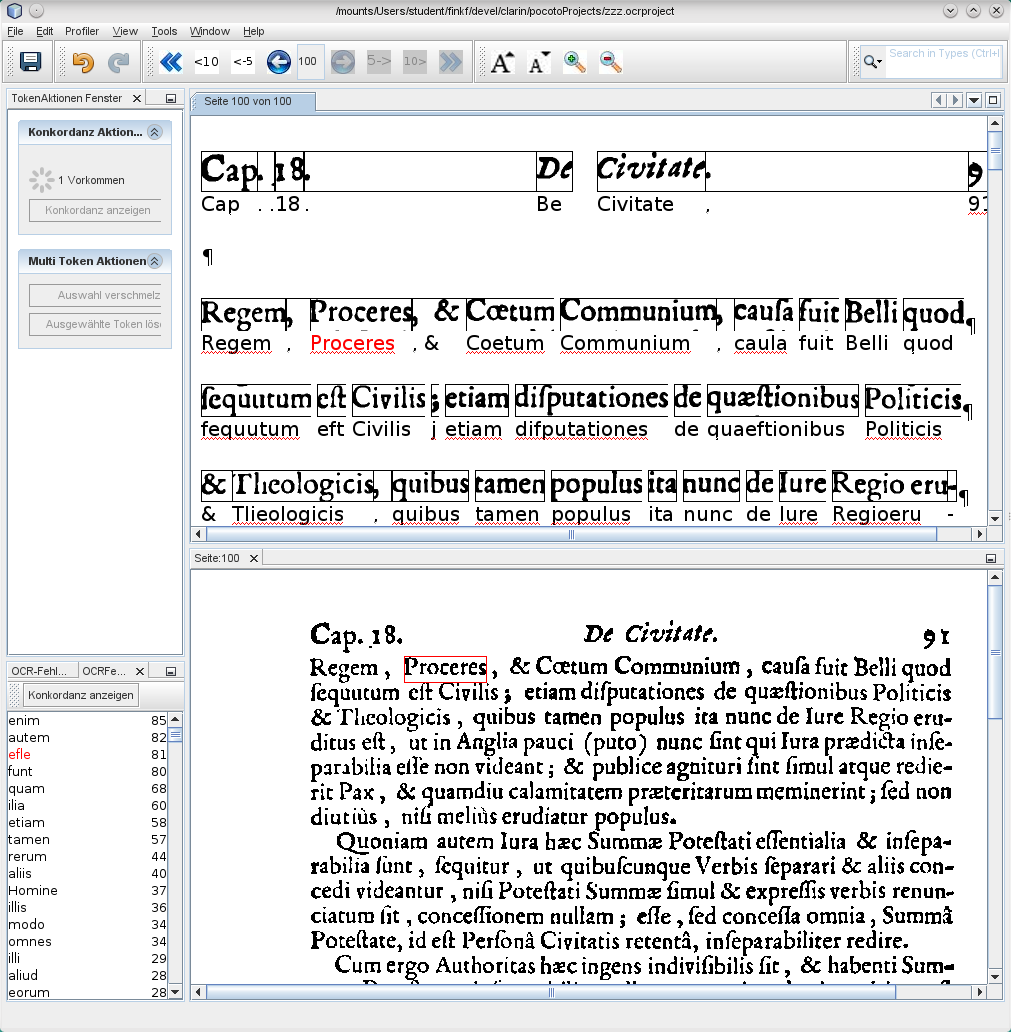
\includegraphics[height=.8\textheight]{../presentations/images/pocoto_ui.png}
		\column{.35\textwidth}
		\begin{itemize}
			\item The token of the text are displayed along with their image details.
			\item The page context shows the active token on the original page.
			\item Error frequencies -- based on the confidence values of the OCR
				engine -- are shown.
		\end{itemize}
	\end{columns}
\end{frame}

\subsection{Creating a concordance view}
\begin{frame}
	\begin{columns}
		\column{.6\textwidth}
		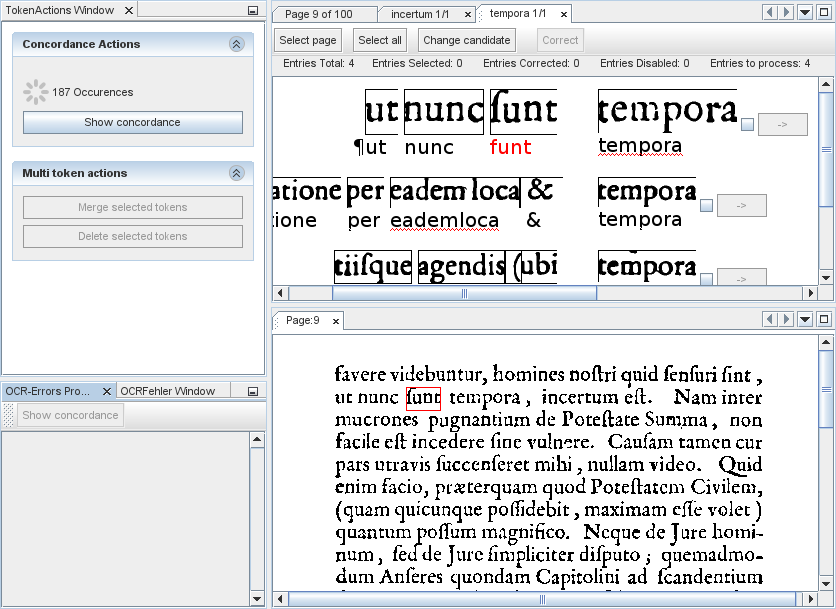
\includegraphics[width=1.0\textwidth]{../presentations/images/concordanceview1.png}
		\column{.35\textwidth}
		\begin{enumerate}
			\item You can activate any token and if there exists any similar other
				token you can click to the \texttt{Show concordance view} button in the
				token action area
			\item You can click on any entry in the two error frequency lists in the
				error area.
		\end{enumerate}
	\end{columns}
\end{frame}

\subsection{Concordance views}
\begin{frame}
	\begin{columns}
		\column{.6\textwidth}
		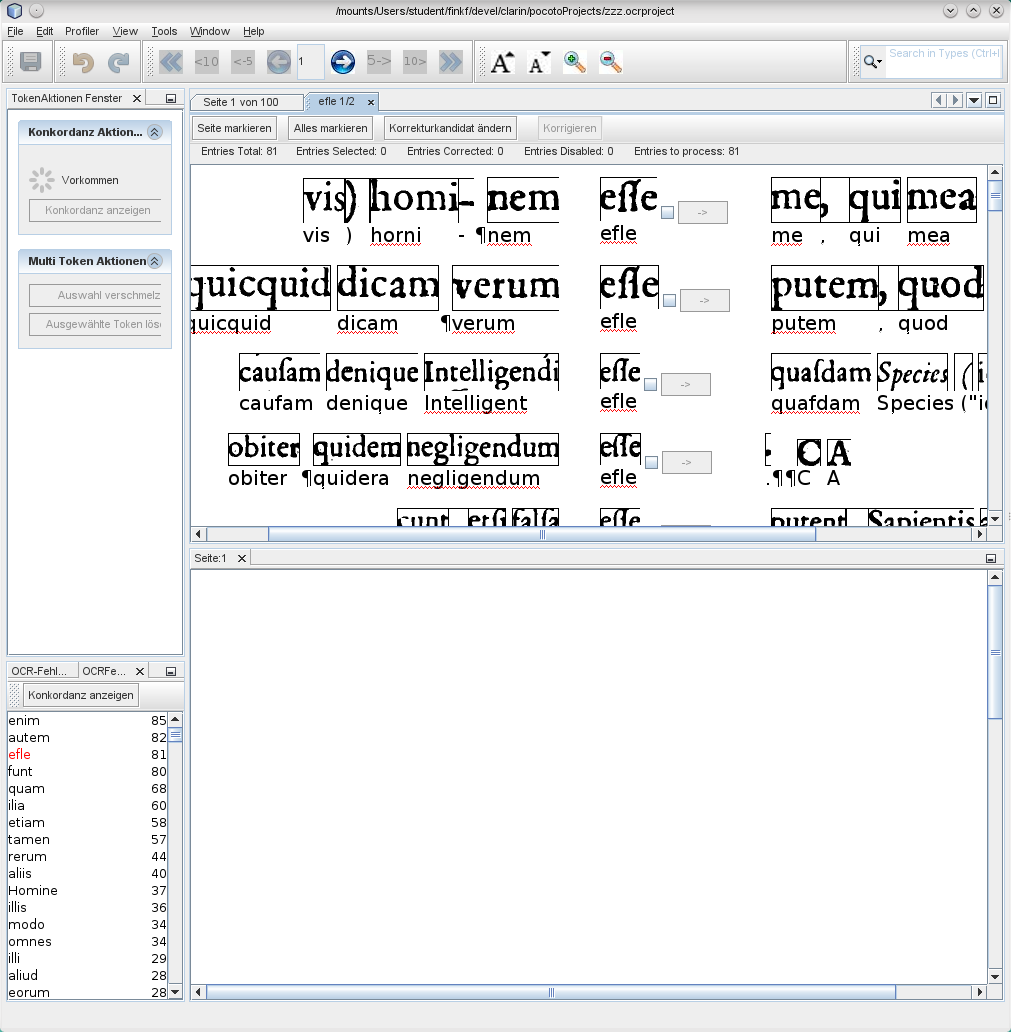
\includegraphics[height=.8\textheight]{../presentations/images/konkordanz_1.png}
		\column{.35\textwidth}
		\begin{itemize}
			\item Common error patterns in the document can be examined using
				the so-called concordance view.
			\item The concordance view lists similar words and patterns
				encountered in the document.
			\item Consistent error patterns can be easily selected and
				corrected in one step.
		\end{itemize}
	\end{columns}
\end{frame}

\section{Interactive post-correction}
\subsection{Overview}
\begin{frame}
	\begin{itemize}
		\item \pocoto{} automatically tokenizes the document on whitespace and
			punctuation.
		\item Each token can be examined in its page image.
		\item \pocoto{} supports the correction of single tokens.
		\item Multiple occurrences of errors and (error patterns) can be corrected
			with concordance views.
		\item Split tokens (Splits) can be merged together.
		\item Merged tokens (Merges) can be split.
	\end{itemize}
\end{frame}

\subsection{correcting single tokens}
\begin{frame}
	\begin{columns}
		\column{.6\textwidth}
		\includegraphics<1>[height=.8\textheight]{../presentations/images/correction_1.png}
		\includegraphics<2>[height=.8\textheight]{../presentations/images/correction_2.png}
		\includegraphics<3>[height=.8\textheight]{../presentations/images/correction_3.png}
		\column{.35\textwidth}
		\begin{itemize}
			\item \emph{Suspicious} words are marked in the text.
			\item Words can be marked as correct.
			\item Words can be merged with their right neighbours.
			\item Words can be corrected manually in the window.
		\end{itemize}
	\end{columns}
\end{frame}

\subsection{Splits and merges}
\begin{frame}
	\begin{columns}
		\column{.6\textwidth}
		\includegraphics<1>[height=.8\textheight]{../presentations/images/merge_1.png}
		\includegraphics<2>[height=.8\textheight]{../presentations/images/merge_2.png}
		\includegraphics<3>[height=.8\textheight]{../presentations/images/merge_3.png}
		\includegraphics<4>[height=.8\textheight]{../presentations/images/split_1.png}
		\includegraphics<5>[height=.8\textheight]{../presentations/images/split_2.png}
		\includegraphics<6>[height=.8\textheight]{../presentations/images/split_3.png}
		\column{.35\textwidth}
		\begin{itemize}
			\item Merged token can be easily split.
			\item Multiple, split token can be easily merged back together.
		\end{itemize}
	\end{columns}
\end{frame}

\subsection{Concordances}
\begin{frame}
	\begin{columns}
		\column{.6\textwidth}
		\includegraphics<1>[height=.8\textheight]{../presentations/images/konkordanz_1.png}
		\includegraphics<2>[height=.8\textheight]{../presentations/images/konkordanz_2.png}
		\includegraphics<3>[height=.8\textheight]{../presentations/images/konkordanz_3.png}
		\includegraphics<4>[height=.8\textheight]{../presentations/images/konkordanz_4.png}
		\includegraphics<5>[height=.8\textheight]{../presentations/images/konkordanz_5.png}
		\column{.35\textwidth}
		\begin{itemize}
			\item Common errors and error patterns in the document can be examined
				using the so-called concordance view.
			\item The concordance view lists similar words and patterns
				encountered in the document.
			\item Consistent errors can be easily selected and corrected in one step.
		\end{itemize}
	\end{columns}
\end{frame}

\section{}
\subsection{}
\begin{frame}
	\centering{
		\Huge Thanks for your attention!
	}
\end{frame}

\end{document}
